\documentclass[aspectratio=169]{beamer}
\usepackage[utf8]{inputenc}
\usepackage{tikz} % for QR code overlay

% code snippets
\usepackage{minted}
\newmintedfile[dockercode]{dockerfile}{
  % bgcolor=mintedbackground,
  fontfamily=tt,
  linenos=true,
  numberblanklines=true,
  numbersep=5pt,
  gobble=0,
  frame=leftline,
  framerule=0.4pt,
  framesep=2mm,
  funcnamehighlighting=true,
  tabsize=4,
  obeytabs=false,
  mathescape=false
  samepage=false, %with this setting you can force the list to appear on the same page
  showspaces=false,
  showtabs =false,
  texcl=false,
}
\newminted[bashcode]{bash}{
  % bgcolor=mintedbackground,
  fontfamily=tt,
  linenos=true,
  numberblanklines=true,
  numbersep=5pt,
  gobble=0,
  frame=leftline,
  framerule=0.4pt,
  framesep=2mm,
  funcnamehighlighting=true,
  tabsize=4,
  obeytabs=false,
  mathescape=false
  samepage=false, %with this setting you can force the list to appear on the same page
  showspaces=false,
  showtabs =false,
  texcl=false,
}

% biblatex (requires biber; sudo pacman -S biber)
\usepackage[]{biblatex} % biblatex
\addbibresource{"./content/bib/bib1.bib"}
\addbibresource{"./content/bib/bib2.bib"}
\addbibresource{"./content/bib/throwaway.bib"}

\usepackage{graphicx}
\graphicspath{ {./content/img/} }

\usetheme{Boadilla}
\usecolortheme{rose}
% \beamerdefaultoverlayspecification{<+->} % this will turn it into slides

\title{Artificial Intelligence, Encrypted Deep Learning, Big Data, and Robots}
\subtitle{New Scientist Live \today}
\author{George Onoufriou\\(University of Lincoln)}
\date{\today}

\begin{document}

\addtobeamertemplate{frametitle}{}{%
\begin{tikzpicture}[remember picture,overlay]
\node[anchor=north east,yshift=2pt] at (current page.north east) {
\includegraphics[height=1.5cm]{qrcode.png}};
\end{tikzpicture}}

  \frame{\titlepage}

  \begin{frame}
    \frametitle{About}
    \begin{columns}
      \begin{column}{0.5\textwidth}
        \begin{itemize}
          \item PhD Candidate Computer/ Data Science
          \item Greek Cypriot
          \item Privacy and Linux Enthusiast
        \end{itemize}
      \end{column}
      \begin{column}{0.5\textwidth}
        \begin{figure}[th!]
          \centering
          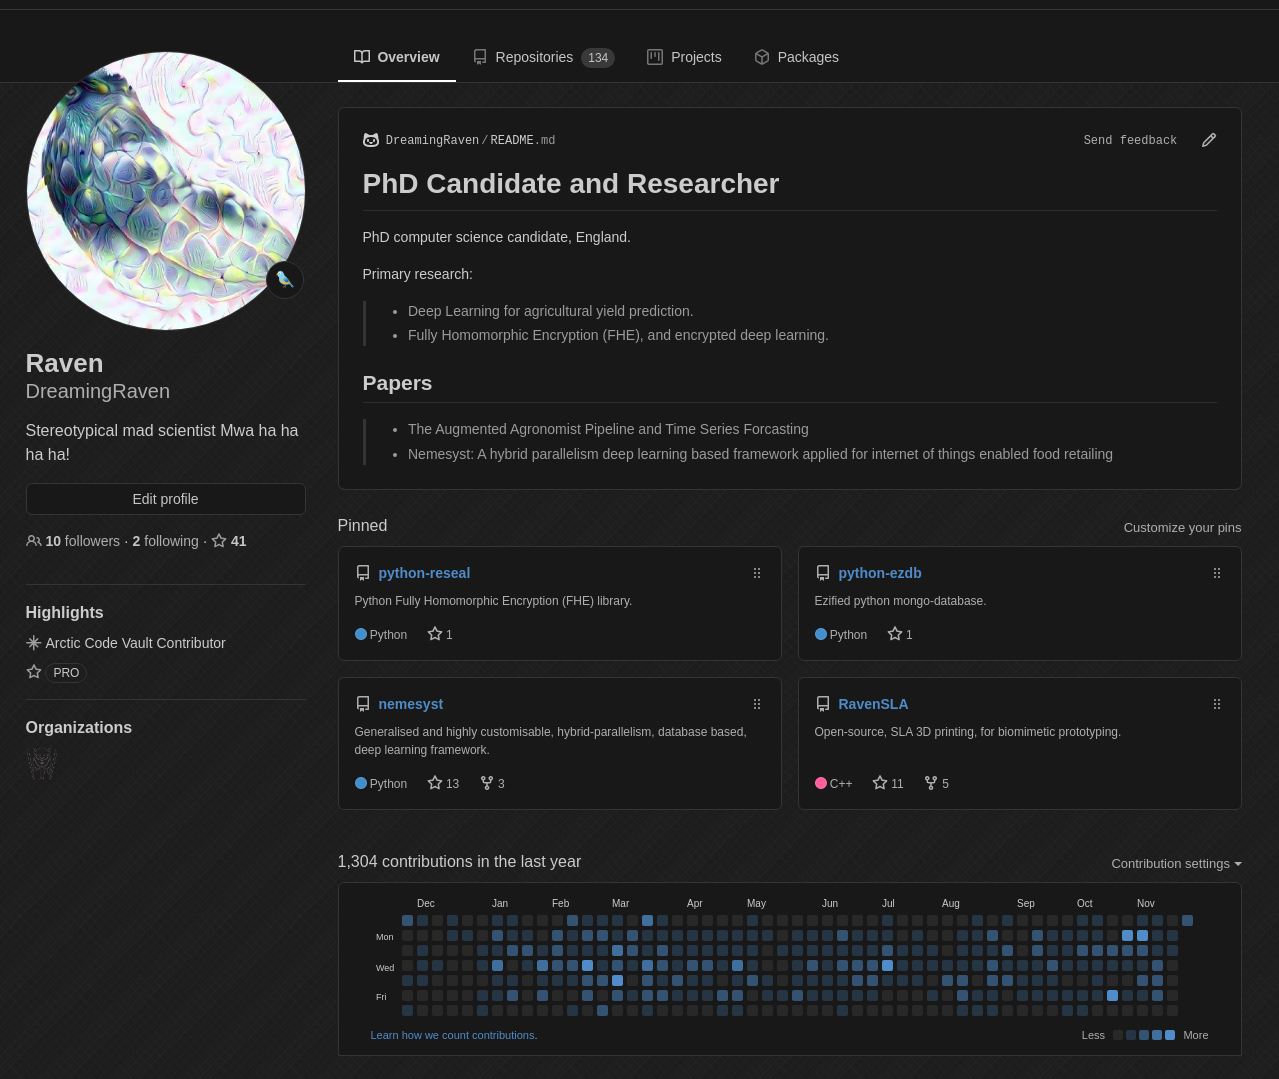
\includegraphics[width=0.8\textwidth]{gh.png}
          \caption{GitHub profile page where you can come to see my work and chat.}
          \label{fig:gh}
        \end{figure}
      \end{column}
    \end{columns}
  \end{frame}

  \begin{frame}
    \frametitle{I Work In}
    \begin{itemize}
        \item Artificial Intelligence
        \item Specifically: Deep Learning (subfield of Artificial Intelligence)
    \end{itemize}
  \end{frame}

  \begin{frame}
    \frametitle{Deep Learning is}
    \begin{itemize}
        \item Machines making sense of the world, and of what they sense, using artificial neurons (brain cells)
        \item We percieve things intuitiveley, but it is quite difficult for a machine
    \end{itemize}
  \end{frame}

  \begin{frame}
    \frametitle{AI/ DL}
    \begin{itemize}
        \item Uses an old model of how we thought neurons in your brain worked
        \item Take in some electrical signals from, eyes, touch, taste ...
        \item Based on these electrical signals, output some related signal ...
        \item We show machines what was supposed to be the output so that they can learn from their mistakes, similarly to what you would expect of a human.
        \item Using layers of these neurons we can become state of the art in almost every field they have been applied to.
        \begin{itemize}
            \item self driving cars
            \item people recognition
            \item medical diagnosis
            \item almost anything you can think of that has the right data
        \end{itemize}
    \end{itemize}
  \end{frame}

  \begin{frame}
    \begin{figure}[th!]
      \centering
      
\includegraphics[width=0.5\textwidth]{docker-is-born-meme.jpg}
      \caption{Docker is born meme.}
      \label{fig:docker_born}
    \end{figure}
  \end{frame}

  \begin{frame}
    \frametitle{How This Worked in Industry}
    \begin{figure}[th!]
      \centering
      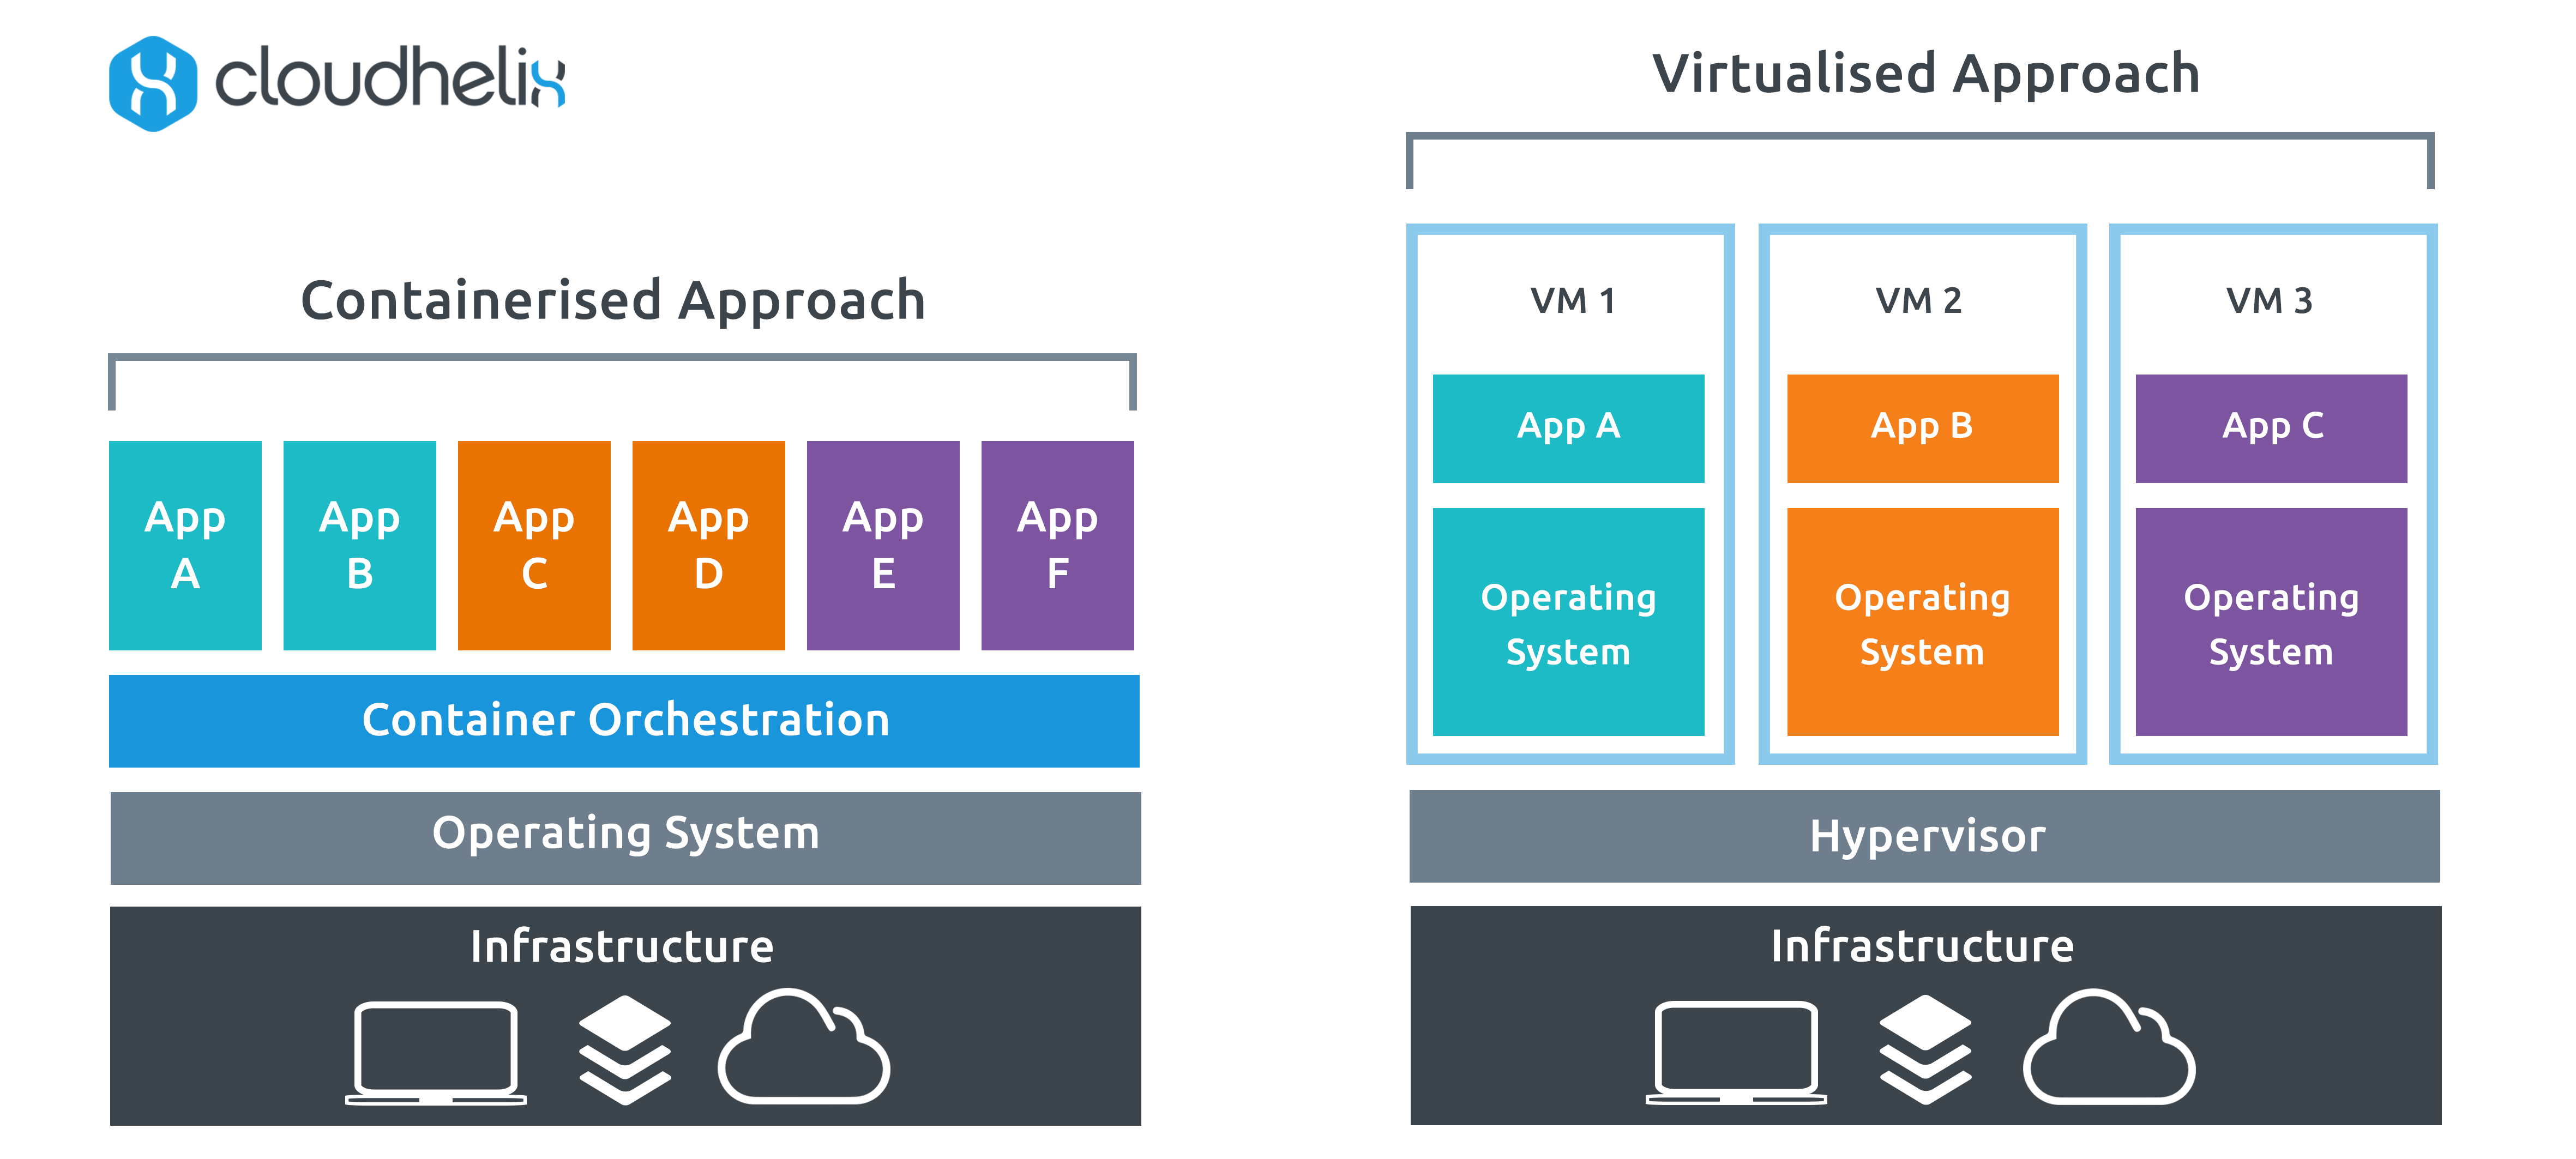
\includegraphics[width=0.9\textwidth]{containerisation.png}
      \caption{Comparing Virtualisation and Containerisation.}
      \label{fig:containerisation}
    \end{figure}
  \end{frame}

  \begin{frame}
    \frametitle{Containerisation Use Cases}
    \begin{figure}[th!]
      \centering
      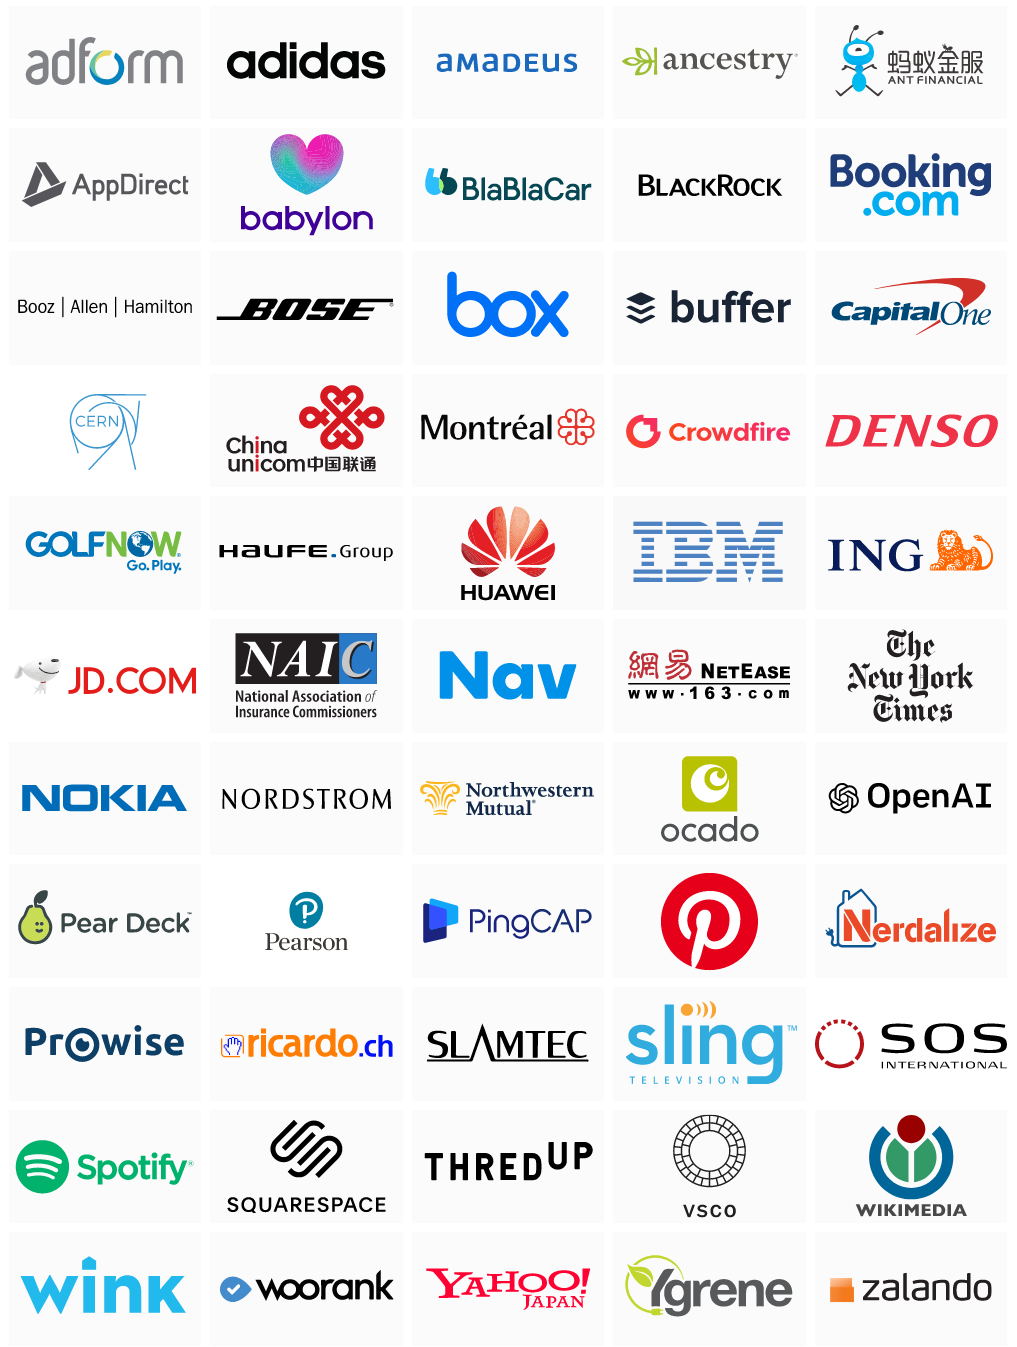
\includegraphics[width=0.4\textwidth]{kube_case_studies.png}
      \caption{Sample Kubernetes use in the wild. \autocite{kube_cases}}
      \label{fig:kube_use}
    \end{figure}
  \end{frame}

  \begin{frame}
    \frametitle{What is Docker}
    \begin{itemize}
        \item Repeatable instructions to (re)create a lightweight virtual machine
    \end{itemize}
    \begin{figure}[th!]
      \centering
      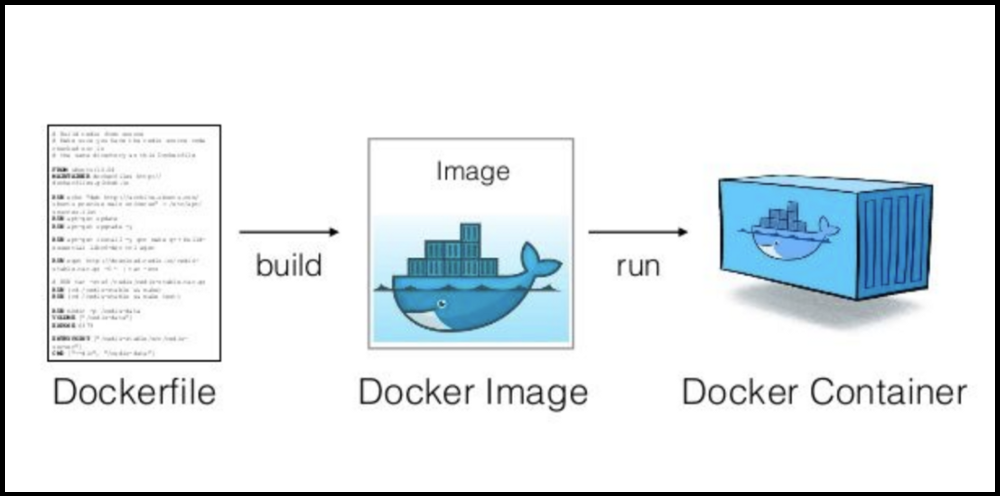
\includegraphics[width=0.7\textwidth]{docker_process.png}
      \caption{Creating Docker Containers. \autocite{docker_build}}
      \label{fig:docker_build}
    \end{figure}
  \end{frame}

  \begin{frame}[fragile]
    \frametitle{Dockerfile build}
    % \inputminted{dockerfile}{content/src/Dockerfile}
    \textbf{\textit{./Dockerfile}}:
    \dockercode{content/src/Dockerfile}
    to build this file (-f Dockerfile) located in this directory ('.') and tag it with name: \textit{"some/tag"}\autocite{docker}:
    \begin{bashcode}
docker build -t some/tag -f Dockerfile .
    \end{bashcode}
  \end{frame}

  \begin{frame}
    \frametitle{Dockerfile Build This Presentation}
    \textbf{\textit{./Dockerfile}}:
    \dockercode{Dockerfile}
  \end{frame}

  \begin{frame}[fragile]% FRAGILE REQUIRED FOR BEAMER + MINTED TO WORK
    \frametitle{Docker Image Use}
    \begin{itemize}
        \item Build a "Dockerfile" file and  tag it as "some/tag":
        \begin{bashcode}
docker build -t some/tag -f Dockerfile .
        \end{bashcode}
        \item Run bash from inside this image known as "some/tag" interactively:
        \begin{bashcode}
docker run -it some/tag bash
        \end{bashcode}
        \item Same as above but now with gpu passthrough and directly calling nvidia-smi to view them
        \begin{bashcode}
docker run --gpus all -it some/tag nvidia-smi
        \end{bashcode}
    \end{itemize}
  \end{frame}

  \begin{frame}
    \frametitle{Docker-Compose}
    \begin{itemize}
        \item Helps reduce command line arguments
        \item Allows source control
        \item Example docker compose included with this presentation
        \item I will now demonstrate ...
    \end{itemize}
  \end{frame}

  \begin{frame}
    \frametitle{Docker Zero to Dev}
    \begin{itemize}
      \item Docker (single container)
      \item Docker-Compose (single node container orchestrator)
      \item Docker Swarm (or other multi node container orchestrator)
    \end{itemize}
    \begin{itemize}
      \item Kubernetes
      \item Apache Mesos
    \end{itemize}
  \end{frame}

  \begin{frame}
      \frametitle{Questions}
      \url{https://github.com/DreamingRaven/2020-docker-talk}
  \end{frame}

  \begin{frame}[allowframebreaks]
    \frametitle{References}
    % % biblatex version
    \printbibliography
  \end{frame}

\end{document}
